\input{preamble.tex}

\moduleAbbr{Ph4I}
\moduleName{Physik 4 für Informatiker}
\license{\ccLogo\,\ccAttribution\,\ccNonCommercial\,\ccShareAlike}

\input{header.tex}

\begin{document}

\input{title.tex}

\section{Elektrostatik}

\subsection{Abkürzungen}

\begin{itemize}
	\item $E$: Elektrische Feldstärke
	\item $\vec{E}$: Elektrisches Feld 
	\item $E_{pot}$: Potentielle Energie
	\item $\varepsilon$: Dielektrizitätskonstante
	\item $\varepsilon_0$: Elektrische Feldkonstante
	\item $\varepsilon_r$: Permittivitätszahl
	\item $\vec{F}$: Kraft
	\item $\vec{p}$: Dipolmoment
	\item $Q$: Ladung
	\item $U$: Elektrische Spannung
	\item $W$: Arbeit
	\item $\varphi$: Elektrisches Potential
	\item $\Phi$: Elektrisches Fluss
\end{itemize}

\subsection{Elektrische Ladung}

Die Ladung 1 Coulomb (C) entspricht der Ladung von $\approx 6.24 \cdot 10^{18}$
Elektronen.

In einem abgeschlossenen System bleibt die Summe aller Ladungen konstant.

\subsection{Coulombsches Gesetz}

Die Kraft $F$ zwischen zwei punktförmigen Ladungen $Q_1$ und $Q_2$ ist umgekehrt
proportional zum Quadrat ihres Abstandes $r$.
\[
	F = a \frac{Q_1Q_2}{r^2}
\]
Dabei ist $a$ eine Konstante die von der Wahl der Ladungseinheit abhängt. Im SI
System ist $a$ folgendermassen festgelegt:
\[
	a = \frac{1}{4 \pi \varepsilon_0}
\]
Hier wiederum ist $\varepsilon_0$ die \textbf{elektrische Feldkonstante}.
\[
	\varepsilon_0 = 8.854 \cdot 10^{-12}
	\quad \left[ \frac{\textrm{C}}{\textrm{V}\cdot \textrm{m}} \right]
\]
Damit erhält das Coulombsche Gesetz folgende Form:
\[
	F = \frac{1}{4\pi\varepsilon_0} \cdot \frac{|Q_1Q_2|}{r^2}
\]
Oder in vektorieller Form, zwischen den zwei Punkten $1$ und $2$:
\[
	\vec{F_{12}} = \frac{1}{4\pi\varepsilon_0}
	\cdot \frac{Q_1Q_2}{|\vec{r_{12}}|^3}
	\cdot \vec{r_{12}}
\]

\subsection{Elektrisches Potential}

Die potentielle Energie pro Ladungseinheit wird als \textit{elektrisches
Potential} bezeichnet.
\[
	\varphi = \frac{1}{Q} E_{pot}
\]
Somit ergibt sich als elektrisches Potential der Punktladung $Q_0$ im Abstand $r$:
\[
	\varphi = \frac{1}{4\pi\varepsilon_0} \frac{Q_0}{r}
\]

\subsection{Elektrische Spannung}
\[
	U_{AB} = \frac{1}{Q} W_{AB} = \int\limits^B_A \vec{E} \cdot d \cdot \vec{s}
\]

\subsection{Ladungsverteilungen}

Ladungen können auch in einem Raumbereich oder auf einer Fläche verteilt sein.

Die Raumladungsdichte $\varrho$ wird folgendermassen definiert:
\[
	\varrho = \frac{Q}{V}
	\quad \left[ \textrm{C}/\textrm{m}^3 \right]
\]
Und die Flächenladungsdichte $\sigma$:
\[
	\sigma = \frac{Q}{A}
	\quad \left[ \textrm{C}/\textrm{m}^2 \right]
\]

\subsection{Elektrisches Feld}

Die elektrische Feldstärke $E$ beträgt:
\[
	E = \frac{F}{Q}
\]

\subsection{Elektrischer Dipol}

Ein elektrischer Dipol besteht aus zwei gleich grossen Punktladungen $Q$
entgegengesetzten Vorzeichens in einem festen Abstand $l$.

Der Dipolmoment $\vec{p}$ ist ein Vektor, er von der negativen Ladung zur
positiven Ladung zeigt und dessen Betrag gleich dem Produkt von Ladung $Q$ und
Abstand $l$ ist:
\[
	|\vec{p}| = Q \cdot l
\]
Das Potential in einem Punkt $P$ (siehe folgende Abbildung) ergibt sich aus der
Summe der zwei einzelnen Potentialen der positiven und negativen Punktladungen.

\begin{center}
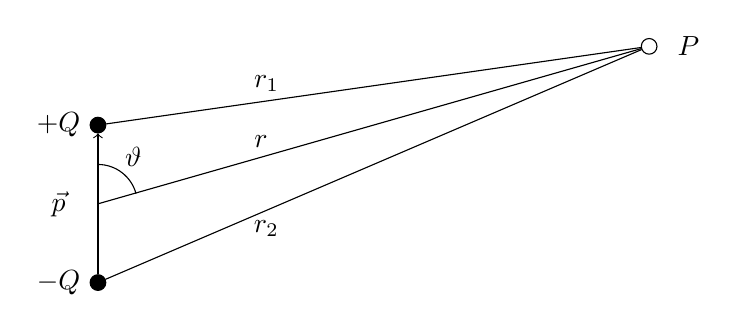
\begin{tikzpicture}
	
	% Styles
	\tikzstyle{dot} = [draw,shape=circle,scale=0.6]
	\tikzstyle{label} = [node distance=5mm]
	\tikzstyle{linelabel} = [pos=0.3,above]

	% Ladungen
	\node at (0,0) [dot,fill=black] (neg) {};
	\node at (0,1) (mom) {};
	\node at (0,2) [dot,fill=black] (pos) {};
	\draw[->] (neg) -- (pos);

	% Labels Ladungen
	\node [label,left of=pos] {$+Q$};
	\node [label,left of=mom] {$\vec{p}$};
	\node [label,left of=neg] {$-Q$};

	% Punkt P mit Verbindungslinien
	\node at (7,3) [dot,fill=white] (P) {};
	\node [label,right of=P] {$P$};
	\draw (pos) -- node [linelabel] {$r_1$} (P);
	\draw (mom.center) -- node [linelabel] {$r$} (P);
	\draw (neg) -- node [linelabel,below] {$r_2$} (P);

	% Winkel
	\draw (0,1.5) arc (90:15:0.5);
	\node at (0.45,1.6) {$\vartheta$};

\end{tikzpicture}

\end{center}

Die Summe der beiden Punktpotentiale ist:
\[
	\varphi
		= \frac{Q}{4\pi\varepsilon_0} \left(\frac{1}{r_1} - \frac{1}{r_2}\right)
		= \frac{Q}{4\pi\varepsilon_0} \frac{r_2 - r_1}{r_1 r_2}
\]
Sofern der Abstand $r$ im Vergleich zum Dipolabstand $l$ gross ist, gilt die
Näherung:
\[
	\varphi = \frac{Q}{4\pi\varepsilon_0} \frac{p}{r^2} \cos \vartheta
\]

\subsection{Gesetz von Gauss}

Der elektrische Fluss durch eine beliebige geschlossene Fläche ist gleich der
Summe der eingeschlossenen Ladungen.
\[
	\Phi = \sum Q
\]

\section{Kondensatoren}

Kapazität:
\[
	C = \frac{Q}{U}
\]

Kapazität Plattenkondensator:
\[
	C = \frac{\varepsilon_0 A}{d}
\]
$d$: Abstand zwischen Platten\\
$A$: Fläche einer Platte

\subsection{Parallel-Schaltung}

Kapazitäten addieren sich.

\begin{minipage}{.5\linewidth}
	\begin{circuitikz}

\draw (1.5,0.5) -- (0,0.5)
	to[C, l=$C_1$] (0,2.5) -- (3,2.5)
	to[C, l=$C_2$] (3,0.5) -- (1.5,0.5) -- (1.5,0) -- (5,0)
	to[battery] (5,3) -- (1.5,3) -- (1.5,0.5)
;

\draw (0,2.5) node[left]{$A$};
\draw (0,0.5) node[left]{$B$};
\draw (3,2.5) node[right]{$C$};
\draw (3,0.5) node[right]{$D$};

\draw (5,2) node[right]{$+$};
\draw (5,1) node[right]{$-$};

\draw (0.5,1.5) node[right]{$U_1$};
\draw (2.5,1.5) node[left]{$U_2$};
\draw (5.5,1.5) node[right]{$C$};

\end{circuitikz}

\end{minipage}
\begin{minipage}{.5\linewidth}
	\begin{align*}
		& C_1 = C_2 \\
		& \Phi_A = \Phi_C \\
		& \Phi_B = \Phi_D \\
		& U = U_1 = U_2 \\
		& Q = Q_1 = Q_2
	\end{align*}
\end{minipage}

\section{Elektrische Ströme}

\textbf{Elektrischer Strom} ist die pro Zeiteinheit durch einen elektrischen Leiter
fliessende Ladung.

TODO formel

\textbf{Stromdichte}:
\begin{align*}
	& j \approx \frac{\textrm{Strom}}{\textrm{Fläche}} \approx \vec{E} \\
	& j = \rho \cdot E = \frac{1}{\rho}E
\end{align*}

\textbf{Elektrische Leitfähigkeit}:
\begin{align*}
	& j = \sigma \cdot \vec{E} \\
	& \sigma = \frac{j}{\vec{E}}
\end{align*}

\textbf{Spezifischer Widerstand}:
\begin{align*}
	& \rho = \frac{1}{\sigma}
\end{align*}

\subsection{Widerstände}

\subsubsection{Innenwiderstand}

Innenwiderstand einer Stromquelle:
\begin{align*}
	& R_i = R \left(\frac{U_0}{U} - 1\right)
\end{align*}

$U_0$: Ohne Last\\
$U$: Mit Last

\subsubsection{Schaltungen}

\begin{minipage}[t]{.5\linewidth}
	Seriell:\\\\
	\begin{circuitikz}

\draw (0,0)
	to[R, l=$R_1$] (2,0)
	to[R, l=$R_2$] (4,0)
	to[R, l=$R_3$] (6,0) -- (6,2) -- (0,2)
	to[battery] (0,0)
;

\end{circuitikz}

\end{minipage}
\begin{minipage}[t]{.5\linewidth}
	Parallel:\\\\
	\begin{circuitikz}

\draw (0,0) -- (0,5)
	to[battery] (3,5) -- (3,0) -- (0,0)
;

\draw (0,3) to[R, l=$R_1$] (3,3);
\draw (0,2) to[R, l=$R_2$] (3,2);
\draw (0,1) to[R, l=$R_3$] (3,1);

\end{circuitikz}

\end{minipage}


\subsection{Kirchhoffsche Regeln}

\subsubsection{Knotenregel}

In einem Knotenpunkt eines elektrischen Netzwerkes ist die Summe der
zufliessenden Ströme gleich der Summe der abfliessenden Ströme.
\[
	\sum_{k=1}^n I_k = 0
\]

\subsubsection{Maschenregel}

Alle Teilspannungen eines Umlaufs bzw. einer Masche in einem elektrischen
Netzwerk addieren sich zu null. Die Richtung des Umlaufes kann beliebig gewählt
werden; sie legt dann aber die Vorzeichen der Teilspannungen fest.
\[
	\sum_{k=1}^n U_k = 0
\]

\section{Arbeit und Leistung}

\begin{align*}
	& P = \frac{dW}{dt} = \frac{dQU}{dt} = U \cdot I = R \cdot I^2 \\
	& W = U \cdot I \cdot t = Q \cdot U \\
	& I = \frac{U_0}{R_i + R} \\
	& P = \left(\frac{U_0}{R_i + R}\right)^2 \cdot R = U_0^2 \cdot R \cdot (R_i + R)^{-2}
\end{align*}

\section{Magnetostatik}

Erstes Ampère'sches Gesetz
\begin{align}
	& \vec{F} = l \cdot \vec{I} \times \vec{B}
\end{align}

Dabei ist $B$ die Magnetische Flussdichte, $H$ die magnetische Feldstärke und
$\mu_0$ die magnetische Feldkonstante.
\begin{align}
	& |B| = \frac{|F|}{l \cdot |I|} \hspace{3em} \\
	& \vec{B} = \mu \cdot \vec{H} = \mu_0 \cdot \mu_r \cdot \vec{H}
\end{align}

Die Einheit der
Magnetischen Flussdichte wird in Tesla gemessen.
\[
	\frac{N}{A \cdot m}
	= \frac{N \cdot m}{A \cdot m^2}
	= \frac{J}{A \cdot m^2}
	= \frac{V \cdot s}{m^2}
	= T
\]


\section{Schwingungen}

\subsection{Trägheitsmomente}

Brett: $\displaystyle\frac{m}{12} \left(h^2 + b^2\right)$

Stab: $\displaystyle\frac{m}{12} l^2$

Für weitere Trägheitsmomente, siehe \textit{Taschenbuch der Physik} von Horst
Kuchling, Seite 132.

\subsection{Pendelschwingungen}

Pendelschwingungen:
\[
	T = 2 \pi \sqrt{\frac{J_S + ma^2}{mga}}	
\]
Dabei ist $T$ die Schwingungsdauer, $J_S$ das Trägheitsmoment und $a$ der
Abstand vom Schwerpunkt.

Die Schwingungsdauer $T$ entspricht der reziproken Frequenz $1/f$. Die
Kreisfrequenz $\omega$ berechnet sich also wie folgt:
\[
	\omega = 2\pi\frac{1}{T}
\]

\subsection{Wellen}

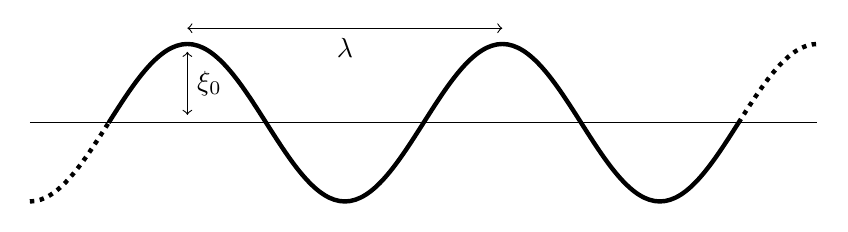
\begin{tikzpicture}

	% Baseline
	\draw (1,0) -- (11,0);

	% Wave
	\draw[x=1cm,y=1cm,dotted,ultra thick] (1,-1) cos (2,0);
	\draw[x=1cm,y=1cm,ultra thick] (2,0)
		sin (3,1) cos (4,0) sin (5,-1) cos (6,0)
		sin (7,1) cos (8,0) sin (9,-1) cos (10,0);
	\draw[x=1cm,y=1cm,dotted,ultra thick] (10,0) sin (11,1);

	% Labels
	\draw[<->] (3,1.2) -- (7,1.2);
	\node[below] at (5,1.2) {$\lambda$};
	\draw[<->] (3,0.1) -- (3,0.9);
	\node[right] at (3,0.5) {$\xi_0$};

\end{tikzpicture}


Frequenz $f$ (manchmal auch als $\nu$ bezeichnet):
\[
	f = \frac{u}{\lambda}
\]
Kreisfrequenz $\omega$:
\[
	\omega = \frac{2 \pi}{T} = 2 \pi f
\]
Wellenlänge $\lambda$:
\[
	\lambda = \frac{2 \pi}{k} = \frac{u}{f}
\]
Wellenzahl $k$:
\[
k = \frac{\omega}{u} = \frac{2 \pi}{\lambda}
\]
Periode, Schwingungsdauer $T$:
\[
	T = \frac{2 \pi}{\omega}
\]
Phase $\varphi$:
\[
	\varphi = \omega t - k x
\]
Phasengeschwindigkeit, Wellengeschwindigkeit $u$:
\[
	u = \frac{\omega}{k} = \lambda f
\]
Auslenkung $\xi$ am Ort $x$ zum Zeitpunkt $t$:
\[
	\xi = \xi_0 \sin (\omega t - k x - \varphi_0)
\]

\subsubsection{Akkustischer Dopplereffekt}

Bewegte Quelle, ruhender Beobachter, kein Winkel:
\[
	f' = \frac{1}{1 \mp \frac{v_Q}{u}} f
\]
Ruhende Quelle, bewegter Beobachter, kein Winkel:
\[
	f' = (1 \pm \frac{v_B}{u}) f
\]
Allgemeine Gleichung mit Winkel $\vartheta$:
\[
	f_B = \frac{u + v_B \cos \vartheta_B}{u - v_Q \cos \vartheta_Q} f_Q
\]

\section{Optik}

\subsection{Reelle / Virtuelle Bilder}

Ein \textbf{reelles Bild} existiert "wirklich", d.h. von dem Ort des Bildes
gehen wirklich Lichtstrahlen aus oder die von einem Objektpunkt ausgehenden
Strahlen haben sich dort getroffen und gehen nun wieder auseinander. Beispiele:
Gemälde, Projektionen, Leinwände oder Fernsehbilder.

Ein \textbf{virtuelles Bild} kann im Gegensatz zu einem reellen Bild nicht auf
einem Schirm abgebildet werden. Es entsteht, wenn sich das Objekt zwischen
Brennpunkt und Linse befindet. Beispiele: Spiegelbilder, Lupe, Mikroskop.


\end{document}
